
\documentclass[english,notitlepage,reprint,nofootinbib]{revtex4-2}  % defines the basic parameters of the document
% If you want a single-column, remove "reprint"

% Allows special characters (including æøå)
\usepackage[utf8]{inputenc}
% \usepackage[english]{babel}

% Note that you may need to download some of these packages manually, it depends on your setup.
% It may be usefult to download TeXMasker, because it includes a large library of the most common packages.

\usepackage{physics,amssymb}  % mathematical symbols (physics imports amsmath)

\usepackage{graphicx}         % include graphics such as plots
\usepackage{xcolor}           % set colors
\usepackage{hyperref}         % automagic cross-referencing

\usepackage{listings}         % display code
\usepackage{subfigure}        % imports a lot of cool and useful figure commands
\usepackage{caption}
\captionsetup{justification=raggedright,singlelinecheck=false}
\usepackage{subcaption}
\captionsetup[subfigure]{labelformat=empty}
% \usepackage{siunitx}

% \usepackage{float}
%\usepackage[section]{placeins}
\usepackage{algorithm}
\usepackage[noend]{algpseudocode}
\usepackage{subfigure}
\usepackage{tikz}
\usetikzlibrary{quantikz2}
% defines the color of hyperref objects
% Blending two colors:  blue!80!black  =  80% blue and 20% black
\hypersetup{ % this is just my personal choice, feel free to change things
    colorlinks,
    linkcolor={red!50!black},
    citecolor={blue!50!black},
    urlcolor={blue!80!black}}


% ===========================================


\begin{document}
\include{amsmath}
\title{Week 39 exercises}  % self-explanatory
\author{Marie Océane Pilskog, Muhammad Mohsin Mumtaz, and Synne Sigstad Jørgensen} % self-explanatory
\date{\today}                             % self-explanatory
\noaffiliation                            % ignore this, but keep it.

%This is how we create an abstract section.
\begin{abstract}
\noindent The aim of Project 1 was to investigate a set of regression methods in great detail. Among these the regression of the following methods have been studied: Ordinary Least Squares (OLS), Ridge, and Lasso. Studies have been performed of bias-variance tradeoff including its derivation, as well as bootstrap and cross-validation. The starting point for the analysis has been the Runge function. The test error was found to minimize at the following degree $\left[\:\:\:\:
\right]$. It was shown that $\left[\:\:\:\: \right]$ is the most effective method for reproducing the closed-form solution. When investigating the Ridge function, an optimal value for the penalty parameter was found at $\left[\lambda = \:\:\:\:
\right]$.         
\end{abstract}
\maketitle


% ===========================================
\section{Introduction}\label{sec:introduction}

 Machine learning $\left(\mathrm{ML}\right)$ is a fast growing field. Today, impacts of the advancements in machine learning are seen in numerous domains such as medicine, humanities, and technology. The principle of Machine Learning is to give us the possibility to find patterns in sets of data without explicitly writing out a specific code for each problem we would like to solve \cite{noauthor_machinelearninguiodocbookmllecturebookpdf_nodate}. The idea is that our generic algorithm can ``learn'' from the data we give it. 

 \subsection{Runges function}
 Runge's funcion, given in \autoref{eq:runges_function} as a classic test case when working with ML. The reason for choosing this function as our function to investigate is a concept we call \textit{Runge's phenomenon}. Discovered by Carl Runge in $1901$ \cite{runges_phenomenon}, the phenomenon describes how when the function is fitted to higher polynomial degrees, we see oscillation at the edges. Using Runge's function is therefore an excellent example to use when one wants to demonstrate that fitting to a higher polynomial degree is not necessarily synonym with improved results. The reason for this is not that polynomial interpolation is an unfit method, but rather a consequence arising from using a high-degree polynomial built from equally spaced points \cite{interpolationcal_runges_2026}. This is something we will go into much further detail in this paper.

 In this paper, we take a deep dive into Runge's function, and its characteristics. We wish to investigate how our models behave when we fit the function with regression, especially focusing on how fitting to higher polynomial degrees affect our results.

\subsection{Methods of Regression}
 One of the desired outputs when working with ML is \textit{regression}: a process where we fit a model to a data set. There are many different approaches to performing regression, some of them we will look at in this paper.

 \textit{Ordinary Least Squares} $\left(\mathrm{OLS}\right)$ is a practical and a fairly straight forward method of regression, where the principle is that you fit your data by minimising the sum of the squared errors \textcolor{red}{should have citation here}. We can solve for the coefficients of a model using \autoref{eq:ols_theta_values}.


 \textit{Ridge} regression follows many of the same principles as the regression with OLS, but we add what we call a \textit{penalty parameter}, to the sqaured lenght of the parameter vector \textcolor{red}{should I have reference here?}. The coefficients can be solved for using \autoref{eq:ridge_theta_values}.


 \textit{Lasso} regression is different from the Ridge Regression model; this one relies on a 1-norm penalty instead of a 2-norm penalty. The model coefficients do not have a closed form solution, but are defined and found by optimising their cost function, defined in \autoref{eq:lasso_cost_function}. Deriving the cost function for Lasso Regression and optimising it gives us \autoref{eq:lasso_optimise}.  


 \subsection{Resampling methods}
 If we have a function $\hat{\theta} = \hat{\theta}(\mathbf{X})$, where $\mathbf{X}$ is random, this means that $\hat{\theta}$ is itself a random variable with an assosiated PDF $p(x)$\cite{noauthor_machinelearninguiodocbookmllecturebookpdf_nodate}. This means that we can draw a certain number of data points from the function, learn our desired characteristics from it, and interpret the results. This can be especially useful if our sample size is small. There are various methods of resampling. The \textit{Bootstrap} method is a method where you draw random samples from your data, with replacement of the drawn observations, from which you can infer statistical quantities. The \textit{Jacknife} method is a method where you purposely leave out one observation at the time, and then drawn new samples. Both methods require independent, identically distributed variables \cite{noauthor_machinelearninguiodocbookmllecturebookpdf_nodate}.

A third method for resampling is the \textit{k-fold cross valiation} method. Here, you organise the splitting between the training data and the test data, to make sure that no samples land in one of the two categories more than any other sample \cite{noauthor_machinelearninguiodocbookmllecturebookpdf_nodate}. You divide the data into so-called $k-folds$, and then the fold serves as the test data, while the remaining data points serve as the training data. 


 \subsection{Optimisers}
 Optimisers are algorithms that change the weights on our model. In this paper, we have used the optimisers \textit{momentum}, \textit{adagrad}, \textit{RMSprop}, and \textit{adam}. These methods are ways of optimising the cost function of our model using different parameters to retrieve better results for our model coefficients.\\ 

 
 This paper is structured as follows: In \autoref{sec:theory} we will present the theoretical background used for our work, as well as relevant equations. In \autoref{sec:methods} we will display the methods we have applied to achieve our results, which will be presented and discussed in \autoref{sec:results_and_discussion}. Our conclusions can be found in \autoref{sec:conclusions}.  

 

 
 The code developed for this paper can be found on our GitHub repository \footnote{link to github}.

\section{Theory}\label{sec:theory}
\textcolor{red}{Note: the theory section will be written more coherent, for now it is just so that the references in the introduction work!}

\subsection{Important equations for regression}
Runge's function is given by
\begin{equation}\label{eq:runges_function}
    f(x) = \frac{1}{1+25x^2}, \qquad x \in [-1, 1].
\end{equation}

When using OLS, we can solve for the model coefficients $\boldsymbol{\hat{\theta}_{\mathrm{OLS}}}$ via the equation 
\begin{equation}\label{eq:ols_theta_values}
    \boldsymbol{\hat{\theta}}_{\mathrm{OLS}} = (\mathbf{X}^{T}\mathbf{X})^{-1}\mathbf{X}^{T}\mathbf{y},
\end{equation}
where $\mathbf{X}$ is the design matrix given by $\boldsymbol{X}\in\mathbb{R}^{n\times p}$ for $n$ observations and $p$ features, $\mathbf{y} \in \mathbb{R}^{n}$ is the function outputs from our descrete data points, and the superscript $T$ means the transpose.

For Ridge regression, we use OLS as our starting point, and then add a penalty parameter, which results in an equation for the parameters given by
\begin{equation}\label{eq:ridge_theta_values}
    \boldsymbol{\hat{\theta}}_{\mathrm{Ridge}} = (\mathbf{X}^{T}\mathbf{X} + \lambda\mathbf{I})^{-1}\mathbf{X}^{T}\mathbf{y},
\end{equation}
where $\mathbf{I}$ is the identity matrix, $\lambda$ is the penalty parameter, and parameters repeating from \autoref{eq:ols_theta_values} have the same meaning.

The cost function for Lasso regression is given by
\begin{equation}\label{eq:lasso_cost_function}
    C(\boldsymbol{\theta}) = \frac{1}{n}||\mathbf{y}-\mathbf{X}\boldsymbol{\theta}||_2^2+\lambda||\boldsymbol{\theta}||_1,
\end{equation}
where $n$ is the amount of data points and $\lambda$ is yet another penalty parameter. Differentiating this function gives us the expression

\begin{equation}\label{eq:lasso_optimise}
   2\mathbf{X}^T\mathbf{X}\boldsymbol{\theta}+\lambda\hspace{0.5mm}\text{sgn}(\boldsymbol{\theta)}=2\mathbf{X}^T\mathbf{y},
\end{equation}
where sgn$(\boldsymbol{\theta})$ is defined as a vector with all the signs of the coefficient vector $\boldsymbol{\theta}$. 


\subsection{The bias-variance tradeoff}
\subsubsection{Bias, variance, and irreducible error}
\textit{Bias} is the difference between the expectation value for the predicted value by our model, and the true value, given by

\begin{equation}\label{eq:bias}
    \mathrm{Bias}{(\hat\theta)} = \mathbb{E}[\hat{\theta}]-\theta,
\end{equation}
where the hat denotes the predicted value, and the \textcolor{red}{plain} $\theta$ is the true value. In other words, the bias is a measure on how simplified our model is \cite{bias_variance_geeksforgeeks}. If the model is oversimplified, it will miss patterns, and ends up underfitting. This happens when we have high bias. When we have lower bias, the model is closer to the true values, and it captures patterns well. \textit{Variance} is an error arising from the model being to sensitive to the training data, which might lead to overfitting as discussed \textcolor{red}{somewhere in the text, make sure this is correct.} The variance is given by 

\begin{equation}\label{eq:variance}
    \mathrm{Var}(\hat{\theta}) = \mathbb{E}[(\hat{\theta}-\mathbb{E}[\hat{\theta}])^2].
\end{equation}
The bias and the variance combine to give us the mean squared error, given by

\begin{equation}\label{eq:mean_square_error}
    \mathrm{MSE} = \mathbb{E}[(\hat{\theta}-\theta)^2].
\end{equation}
 The irreducible error $\sigma^2$ is a variance of the noise. Because the noise is random, will $\sigma^2$ be a floor beneath the test error. This means that the total test error is a combination of the bias, the variance, and this irreducible error:
 
\begin{equation}\label{eq:total_test_error}
    \mathrm{test\:error} = \mathrm{bias} + \mathrm{variance} + \sigma^2.
\end{equation}

The \textit{bias-variance tradeoff} describes the balance between the bias and the variance. A simplified model leads to a bias increase, but a variance decrease, because the model is not too sensitive to the training data. On the other hand, if we make the model complex the bias is lowered, but the variance error is larger, because we have now fit very closely to the training data. The goal is to find a middleground between these errors.    

\subsubsection{The bias-variation trade-off derivation}
Assume you have a noisy model $\mathbf{y}=f(\mathbf{x})+\boldsymbol{\varepsilon}$, where $\varepsilon \sim N(0, \sigma^2)$. Further assume that you have a data set $\tilde{y}$ predicts $y$, we try to find the expected value of the mean square error $\displaystyle E[(\mathbf{y}-\mathbf{\tilde{y}})^2]$. \textcolor{red}{not done yet...}

\subsection{Scaling and intercept}\label{eq:scaling_and_intercept}
Sometimes, the data we use in our model have very different orders of magnitude, or different units. For example, if we have a data set of distances, where some measurements are in the units of meters and some are in the units of kilometers, the measurements will be penalised differently. Centerting and scaling of the data effectively make the input features comparable! \textcolor{red}{used chat gpt here for explanations}. When they are, the penalty can treat them more fairly. It is common to scale the desig matrix so that evry column has zero mean and unit standard deviation, using

\begin{equation}\label{eq:scaling_X}
    x_j^{(i)} \rightarrow \frac{x_j^{(i)}-\overline{x}_j}{\sigma(x_j)},
\end{equation}
where $x$ is a measurement, $i$ denotes the row, $j$ denotes the column, the overline denotes the mean, and $sigma$ is the standard deviation. In addition to scaling the design matrix, we should also center the $y$-values. When we do this, we essensially remove the intercept, so we no longer have a baseline level for our model. The scaling of the $y$-values can simply be done as

\begin{equation}\label{eq:centering_y}
    y_j = y_j - \overline{y}_j.
\end{equation}

\section{Methods}\label{sec:methods}
\input{sections/methods.tex}

\section{Results and Discussion}\label{sec:results_and_discussion}

\subsection{Mean Square Error, $R^2$ score, and optimal polynomial degree}

\autoref{fig:results_mse_values} shows us the MSE values and $R^2$ scores for our chosen range of  polynomial degrees. For the training data, we find from the MSE values that the optimal polynomial degree is $14$, while for the test data we find a polynomial degree $7$. This difference is expected, as for the training MSE values we train our model on a certain set of noise values, and the higher the polynomial the better the fit for that specific noise data set. However, when we then use the trained model to fit for the test data with new noise data points, the model is fitted so closely with the noise data points for the training data, that the model may no longer be a good fit for the test data. This is what we call \textit{overfitting}, and shows us that the highest polynomial degree is not necessarily the best one.

$R^2$ is the dimentionless \textit{coefficient of determination}, and it compares the model against the best constant 
prediction \cite{noauthor_machinelearninguiodocbookmllecturebookpdf_nodate}. The closer to $1$ the better the fit, and the closer to $0$, the worse the model. 

\begin{figure}[h!]
    \centering
    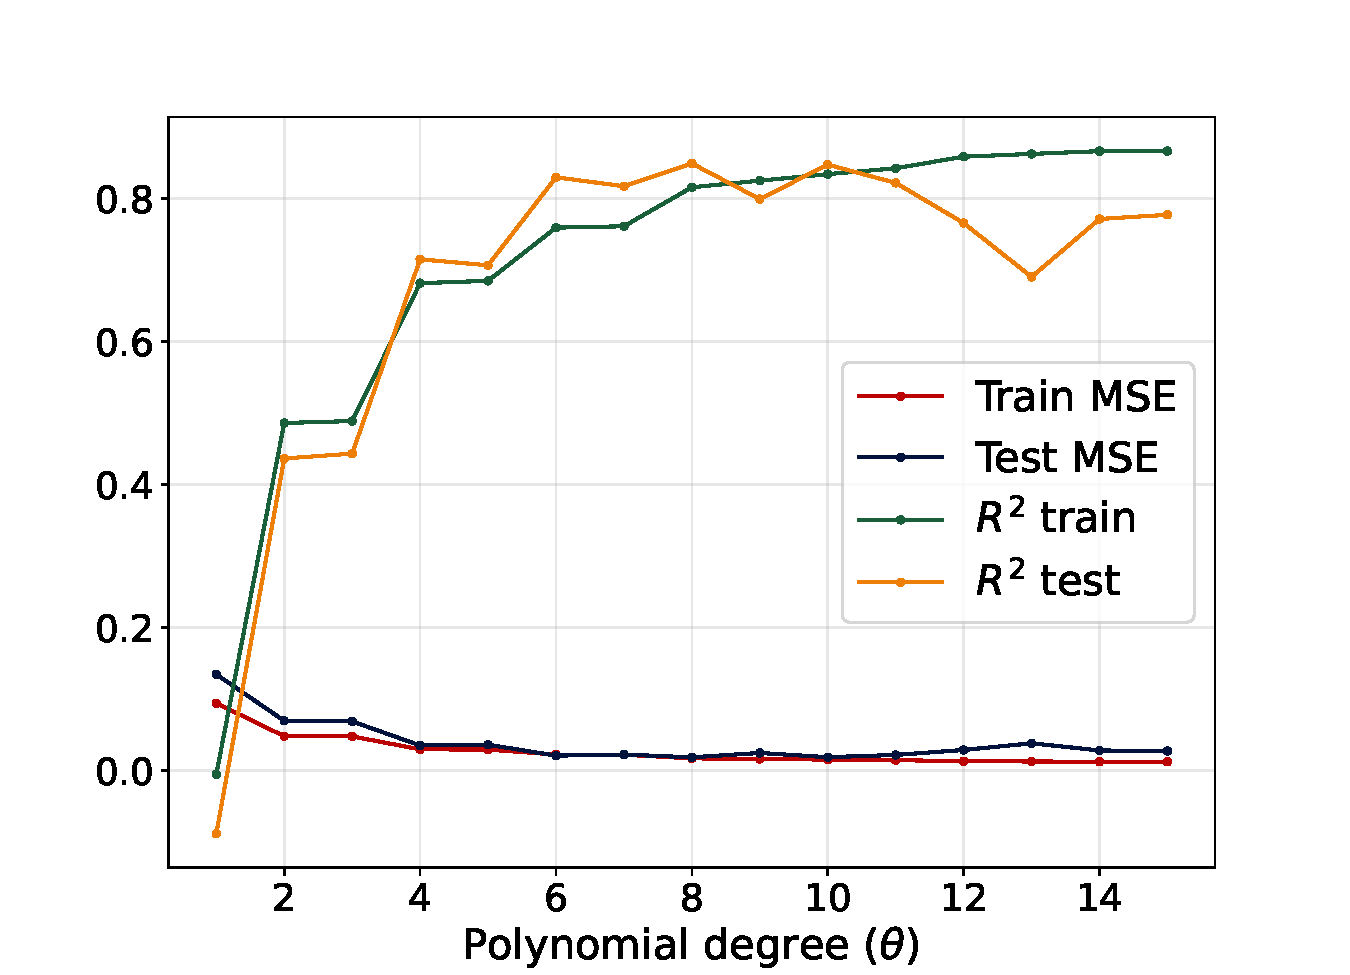
\includegraphics[width = 1.0\linewidth]{../figures/mse_values.pdf}
    \caption{Caption}
    \label{fig:results_mse_values}
\end{figure}

\section{Conclusions}\label{sec:conclusions}
\textcolor{red}{the conclusion is still very general, as we havent finished the exercises for the project. We will aim  to present much more direct results once the exercises have been solved.}\\

We have in this paper performed a comprehensive and thorough analysis of regression, resampling, and optimisation. With the Runge function as a classical test function and starting point, we have visited OLS, Ridge, and Lasso regression, and looked at the mean square error, and the penalty parameter $\lambda$. We found that for our function, the optimal polynomial degree is $2$. We have visited multiple resampling methods, namely the \textit{bootstrap} method and the \textit{k-fold cross validation} method. We have also investigated various optimisation algorithms, and found that the so-called \textit{adam} algorithm was the least sensitive to $\lambda$.  

Topics for further work include ...


\section{Figures}\label{sec:figures}
\input{sections/figures.tex}



% ===========================================

%\newpage
\onecolumngrid
\bibliographystyle{unsrt}
\bibliography{references}

\newpage
\appendix
\section{Use of AI/LLM Tools}
In our work for project 1, we have written the code ourselves and have not used any AI or LLM Tools for generating code or text. 
\subsection{Tools used}
No use of AI/LLM tools.
\subsection{Text writing and editing}
The report has level 0 of AI/LLM tool use.
\subsection{Code generation and assistance}
The developed code has level 0 of AI/LLM tool use.

\end{document}
